\documentclass[tikz,border=2pt]{standalone}
\usepackage{amsmath,amssymb}
\usetikzlibrary{arrows.meta,decorations.pathreplacing}
\begin{document}
% Mixed-strategy example: prior p=0.2 on C, q_C=1, q_W=1/2. Entry has probability
% 0.2 + 0.8*0.5 = 0.6, of which 0.2 comes from C, so mu = P(C | entry) = 0.2/0.6 = 1/3.
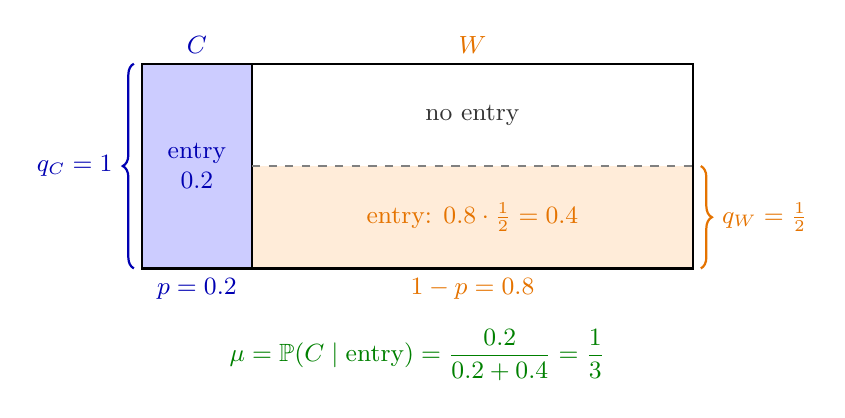
\begin{tikzpicture}[font=\small, >={Latex[length=2mm]}]
  \def\H{2.6}
  % entry regions
  \fill[blue!20] (0,0) rectangle (1.4,\H);
  \fill[orange!15] (1.4,0) rectangle (7.0,0.5*\H);
  % outline and split
  \draw[thick] (0,0) rectangle (7.0,\H);
  \draw[thick] (1.4,0) -- (1.4,\H);
  \draw[thin, dashed, gray] (1.4,0.5*\H) -- (7.0,0.5*\H);
  % type labels
  \node[blue!70!black, anchor=south] at (0.7,\H) {$C$};
  \node[orange!90!black, anchor=south] at (4.2,\H) {$W$};
  \node[blue!70!black, anchor=north] at (0.7,0) {$p=0.2$};
  \node[orange!90!black, anchor=north] at (4.2,0) {$1-p=0.8$};
  % areas
  \node[blue!70!black, align=center] at (0.7,0.5*\H) {entry\\$0.2$};
  \node[orange!90!black] at (4.2,0.25*\H) {entry: $0.8\cdot\tfrac12=0.4$};
  \node[gray!40!black] at (4.2,0.75*\H) {no entry};
  % q_W brace
  \draw[decorate, decoration={brace, amplitude=4pt}, orange!90!black, thick]
    (7.1,0.5*\H) -- node[right, xshift=4pt] {$q_W=\tfrac12$} (7.1,0);
  \draw[decorate, decoration={brace, amplitude=4pt}, blue!70!black, thick]
    (-0.1,0) -- node[left, xshift=-4pt] {$q_C=1$} (-0.1,\H);
  % posterior
  \node[green!50!black, anchor=north] at (3.5,-0.65) {$\mu=\mathbb P(C\mid\text{entry})=\dfrac{0.2}{0.2+0.4}=\dfrac13$};
\end{tikzpicture}
\end{document}
